\chapter{An Investigation into the Security of RobotWeb}
This chapter will investigate the behaviour of the RobotWeb when it is under attack. We will start by definining the expected behaviour of an attacker, including its incentives to attack. From then, we will construct and examine a simplified version of the RobotWeb to determine how victims of an attack will behave. Finally, we present and test several hypotheses about the behaviour of the RobotWeb under attack.

\section{The behaviour of an ideal attacker}
In order to predict the nature of an attacker's behaviour, we must first understand how normal robots behave in the RobotWeb. At all times, a robot will have a noisy estimate of its current position, as it moves the associated noise will grow. When robot $r_1$ encounters another $r_2$, it measures it and creates a factor between its own and $r_2$'s current pose variable. Both robots will then exchange messages to each other over the factor, both using the messages to improve their own location estimates and decrease their uncertainty. In addition to other robots, a robot may measure a fixed beacon, which once again creates a factor between them, however, here only the robot will update its position estimate, as the beacon does not move. The quality of all sent message is dependent on the sender's own position accuracy and the accuracy of its sensors.

An attacker can take the form of either another robot or a beacon in the RobotWeb. Regardless of the form taken by the attacker, its goal would be to control the other robots' position estimates, by sending specially crafted messages.

All robots require a method to localise themselves as part of their normal operations, even attackers. Normal robots use the RobotWeb to do this, while we have no guarantees on the methods that potential attackers may use. An attacker may use an external system for localisation, or even a private RobotWeb, which renders it impervious to any consequences for its actions. However, some attackers may instead choose to participate in the RobotWeb in order to avoid the complexity of using an alternative system. Participating attackers would then have incentive to partially preserve the RobotWeb as they themselves are dependent on it. This dependency is likely cause attackers to only attack a small subset of robots, or only attack robots for a small amount of time. 

It is self-evident that all attackers would seek to be effective i.e. thier attacks should have a high chance of working especially when no defences are present. In seeking effectiveness in the face of defences, attackers should not want their attacks to be easily identified, as identified attacks can be easily defended against. Thus it stands to reason that attacks are likely to be subtly executed, such that their victims would be able to believe them. For example, an attack that suggests that a small robot has moved 10km in 5s is guaranteed to fail.

Finally, in the event that multiple attackers are present in the environment, they would do best to collaborate rather than compete, as it would raise the effectiveness of them all. Since competing attackers are less effective than collaborating attackers, we shall spend less time considering them.

\section{A simplified system}
Any theoretical investigation of the RobotWeb would require the investigator to analyse its backbone, the factor graph. However, the investigator would soon find themselves ensnared by complexity; caught in an intricate web of variable and factor nodes; messages constantly scurrying between them. Worse yet, the web would constantly be spun and unspun as robots moved closer and further from each other.
In the face of this complexity, it becomes clear that a simplification is needed.

To start, we choose to limit our investigation to a single variable, chosen arbitrarily, in the factor graph. Fortunately, the properties of Belief Propagation allow us to reason about this variable without loss of generality. Equation \ref{eqn:bp_belief} shows that the belief of a given variable is solely dependent on its connected factors. 

\begin{figure}[!h]
	\centering
	

\tikzset{every picture/.style={line width=0.75pt}} %set default line width to 0.75pt        

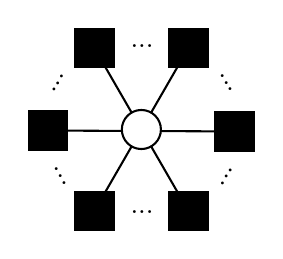
\begin{tikzpicture}[x=0.75pt,y=0.75pt,yscale=-1,xscale=1]
%uncomment if require: \path (0,288); %set diagram left start at 0, and has height of 288

%Shape: Square [id:dp5011100430912303] 
\draw  [fill={rgb, 255:red, 0; green, 0; blue, 0 }  ,fill opacity=1 ] (221.44,121.44) -- (240,121.44) -- (240,140) -- (221.44,140) -- cycle ;
%Shape: Square [id:dp1834276888413744] 
\draw  [fill={rgb, 255:red, 0; green, 0; blue, 0 }  ,fill opacity=1 ] (199.12,159.78) -- (217.68,159.78) -- (217.68,178.34) -- (199.12,178.34) -- cycle ;
%Shape: Square [id:dp4346063530366504] 
\draw  [fill={rgb, 255:red, 0; green, 0; blue, 0 }  ,fill opacity=1 ] (199.12,81.22) -- (217.68,81.22) -- (217.68,99.78) -- (199.12,99.78) -- cycle ;
%Straight Lines [id:da04926983509243965] 
\draw    (230.72,130.72) -- (140.72,130.28) ;
%Straight Lines [id:da6042872004378272] 
\draw    (208.4,169.06) -- (163.04,90.5) ;
%Straight Lines [id:da23454228445560488] 
\draw    (163.04,169.06) -- (208.4,90.5) ;
%Shape: Circle [id:dp7060474924289566] 
\draw  [fill={rgb, 255:red, 255; green, 255; blue, 255 }  ,fill opacity=1 ] (176.31,129.78) .. controls (176.31,124.59) and (180.53,120.37) .. (185.72,120.37) .. controls (190.91,120.37) and (195.13,124.59) .. (195.13,129.78) .. controls (195.13,134.97) and (190.91,139.19) .. (185.72,139.19) .. controls (180.53,139.19) and (176.31,134.97) .. (176.31,129.78) -- cycle ;
%Shape: Square [id:dp12209236616988428] 
\draw  [fill={rgb, 255:red, 0; green, 0; blue, 0 }  ,fill opacity=1 ] (131.44,121) -- (150,121) -- (150,139.56) -- (131.44,139.56) -- cycle ;
%Shape: Square [id:dp4564996494162272] 
\draw  [fill={rgb, 255:red, 0; green, 0; blue, 0 }  ,fill opacity=1 ] (153.76,159.78) -- (172.32,159.78) -- (172.32,178.34) -- (153.76,178.34) -- cycle ;
%Shape: Square [id:dp4857190958072921] 
\draw  [fill={rgb, 255:red, 0; green, 0; blue, 0 }  ,fill opacity=1 ] (153.76,81.22) -- (172.32,81.22) -- (172.32,99.78) -- (153.76,99.78) -- cycle ;

% Text Node
\draw (225,100) node [anchor=north west][inner sep=0.75pt]  [rotate=-60] [align=left] {...};
% Text Node
\draw (221.25,157.5) node [anchor=north west][inner sep=0.75pt]  [rotate=60] [align=left] {...};
% Text Node
\draw (179,87.5) node [anchor=north west][inner sep=0.75pt]   [align=left] {...};
% Text Node
\draw (145,145) node [anchor=north west][inner sep=0.75pt]  [rotate=-60] [align=left] {...};
% Text Node
\draw (179,167.5) node [anchor=north west][inner sep=0.75pt]   [align=left] {...};
% Text Node
\draw (140,112.5) node [anchor=north west][inner sep=0.75pt]  [rotate=60] [align=left] {...};


\end{tikzpicture}

	\caption[Single Variable in a Factor Graph]{A single variable connected to a number of factors}
\end{figure}

One problem still remains with the above setup - a single variable can be connected to any number of factors. As a further simplification, we can group the factors together based off their shared characteristics, which include their origin (if they are internal to the robot or not), their type (what kind of sensor they represent) and their intentions (whether they will help or hinder the robot). For our purposes, we will split the set of factors $F$, into sets $G$ and $B$ based off whether the factors are ``good'' or ``bad'' for the robot. Good factors aim to steer the variable towards the a ground truth value, while bad factors aim to steer it away. Notice that the sets $G$ and $B$ form a cover of $F$, that is $F = G \cup B$.

We then take this a step further and replace each set of factors with a single ``representative factor''.
\begin{figure}[!ht]
	\centering
	

\tikzset{every picture/.style={line width=0.75pt}} %set default line width to 0.75pt        

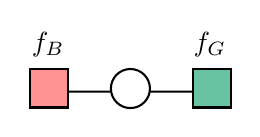
\begin{tikzpicture}[x=0.75pt,y=0.75pt,yscale=-1,xscale=1]
%uncomment if require: \path (0,171); %set diagram left start at 0, and has height of 171

%Straight Lines [id:da9426074160582016] 
\draw    (399.22,143.78) -- (359.94,143.66) ;
%Straight Lines [id:da643000004312603] 
\draw    (399.22,143.78) -- (438.5,143.66) ;
%Shape: Circle [id:dp3724334158586291] 
\draw  [fill={rgb, 255:red, 255; green, 255; blue, 255 }  ,fill opacity=1 ] (389.81,142.22) .. controls (389.81,137.03) and (394.02,132.81) .. (399.22,132.81) .. controls (404.41,132.81) and (408.62,137.03) .. (408.62,142.22) .. controls (408.62,147.41) and (404.41,151.63) .. (399.22,151.63) .. controls (394.02,151.63) and (389.81,147.41) .. (389.81,142.22) -- cycle ;
%Shape: Square [id:dp37804195853429245] 
\draw  [fill={rgb, 255:red, 255; green, 147; blue, 147 }  ,fill opacity=1 ] (350.66,132.81) -- (369.22,132.81) -- (369.22,151.37) -- (350.66,151.37) -- cycle ;
%Shape: Square [id:dp19659269496953535] 
\draw  [fill={rgb, 255:red, 104; green, 195; blue, 163 }  ,fill opacity=1 ] (429.22,132.81) -- (447.78,132.81) -- (447.78,151.37) -- (429.22,151.37) -- cycle ;

% Text Node
\draw (428.22,113.4) node [anchor=north west][inner sep=0.75pt]    {$f_{G}$};
% Text Node
\draw (350.22,113.4) node [anchor=north west][inner sep=0.75pt]    {$f_{B}$};


\end{tikzpicture}


	\caption[Representative factor graph around a single variable]{The above factor graph using ``representative factors''. $f_G$ and $f_B$ respectively represent the sets of good factors ($G$) and bad factors ($B$).}
\end{figure}

We calculate the messages from each of these representative factors as such:
\begin{eqnarray}
	m_{f_G \rightarrow x_i} = \underset{g \in G}{\prod} m_{f_g \rightarrow x_i}&
	m_{f_B \rightarrow x_i} = \underset{b \in B}{\prod} m_{f_b \rightarrow x_i}
\end{eqnarray}
Thus the belief of the variable becomes $p(x) = m_{f_G \rightarrow x} m_{f_B \rightarrow x}$, and since $G \cup B$ covers every factor connected to the variable, we can show that this replacement can be made without altering the variable's final result by equation \ref{eqn:bp_belief}.

\begin{equation}
	p(x_i) = \underset{s \in N(i)}{\prod} m_{f_s \rightarrow x_i}
	\tag{\ref{eqn:bp_belief}}
\end{equation}

For completeness we now present the equations for contents of the messages $m_{f_G \rightarrow x_i}$ and $m_{f_B \rightarrow x_i}$. 
Each message is has an information vector $\eta$ and a precision matrix $\Lambda$.
\begin{eqnarray}
	\eta_G = \underset{g \in G}{\sum} \eta_g&
	\Lambda_G = \underset{g \in G}{\sum} \Lambda_g \label{eqn:good_pull}\\
	\eta_B = \underset{b \in B}{\sum} \eta_b&
	\Lambda_B = \underset{b \in B}{\sum} \Lambda_b \label{eqn:bad_pull}
\end{eqnarray}

\section{Theoretical properties of the RobotWeb under attack}
\subsection{Measuring the strength of an attack}
From the above setup we will now aim to quantify the strength of an attack. For mathematical convenience and ease of understanding, we will derive these equations in 1 dimension, and later present the n-dimensional forms.

To measure the strength of an attack we want to understand the impact of the bad factors on the variable's final belief. To do this we shall use the Kullback-Leibler (KL) divergence \citationneeded between the variable's belief when it is safe and when it is under attack.
The KL divergence is a measure of far the distribution Q is from the distribution P. The further the belief distribution under attack (BDA) is from the distribution suggested by the good factors, the stronger we say the attack is. Similarly, the closer the BDA is to the distribution suggested by the bad factors, the stronger the attack.

The KL divergence between 2 distributions of continuous random variables is:
\begin{equation}
	D_{KL}(P || Q) = \int_{-\infty}^{\infty} log\left( \frac{p(x)}{q(x)} \right) dx
\end{equation}

However a special case exists for Normal distributions, $N_1(\mu_1, \sigma_1^2)$ and $N_2(\mu_2, \sigma_2^2)$.
\begin{equation}
	D_{KL}(N_1 || N_2) = log\left(\frac{\sigma_2}{\sigma_1}\right) + \frac{\sigma_1^2 + (\mu_1 - \mu_2)^2}{2\sigma_2^2} - \frac{1}{2}
\end{equation}

In 1 dimension the messages sent from $f_G$ and $f_B$ are:
\begin{eqnarray}
	m_{f_G \rightarrow x_i} = (\eta_G, \Lambda_G) = (\frac{\mg}{\sgsq}, \frac{1}{\sgsq})\\
	m_{f_B \rightarrow x_i} = (\eta_B, \Lambda_B) = (\frac{\mb}{\sbsq}, \frac{1}{\sbsq}) \label{eqn:attacker_msg}
\end{eqnarray}

From \ref{eqn:bp_belief} we see that the BDA is equal to:
\begin{align}
	m_{f_G \rightarrow x} m_{f_B \rightarrow x} 
	&= (\eta_G + \eta_B, \Lambda_G + \Lambda_B)\\
	&= \left(\frac{\mg}{\sgsq} + \frac{\mb}{\sbsq}, \frac{1}{\sgsq} + \frac{1}{\sbsq}\right)\\
	&= \left(\frac{\mg\sbsq + \mb\sgsq}{\sgsq \sbsq}, \frac{\sbsq + \sgsq}{\sgsq \sbsq}\right)
\end{align}

The above distributions follow the following Normal distributions:
\begin{align}
	G &\sim N\left(\frac{\eta_G}{\Lambda_G}, \frac{1}{\Lambda_G}\right)\\
	B &\sim N\left(\frac{\eta_B}{\Lambda_B}, \frac{1}{\Lambda_B}\right)\\
	BDA &\sim N\left(\mu_{BDA}, \sigma_{BDA}^2\right)\\
	&\sim N\left(\frac{\eta_G + \eta_B}{\Lambda_G + \Lambda_B}, \frac{1}{\Lambda_G + \Lambda_B}\right)\\
	&\sim N\left(\frac{\mg\sbsq + \mb\sgsq}{\sgsq + \sbsq}, \frac{\sgsq \sbsq}{\sgsq + \sbsq}\right) \label{eqn:bda_distribution}
\end{align}

So now we take the KL divergence between the good factors' distribution $G$ and BDA. To make this easier to follow we derive each term in the sum separately.

First deriving the log term we get:
\begin{align}
	log\left(\frac{\sigma_{BDA}}{\sigma_{G}}\right)
	&= log\left(\sqrt[2]{\frac{\sigma_{BDA}^2}{\sigma_{G}^2}}\right)\\
	&= \frac{1}{2} log\left(\frac{\sigma_{BDA}^2}{\sigma_{G}^2}\right)\\
	&= \frac{1}{2} log\left(\frac{\sgsq \sbsq}{\sbsq + \sgsq} \times \frac{1}{\sgsq}\right)\\
	&= \frac{1}{2} log\left(\frac{\sbsq}{\sbsq + \sgsq}\right)
\end{align}

Next we derive the fractional term:
\begin{align}
	\frac{\sigma_{G}^2 + (\mu_{G} - \mu_{BDA})^2}{2\sigma_{BDA}^2}
	&= \frac{
			\sgsq + \left(\mg - \frac{\mg\sbsq + \mb\sgsq}{\sbsq + \sgsq}\right)^2
		}{
			2 \frac{\sgsq \sbsq}{\sbsq + \sgsq}
		}\\
	&= \left(\sgsq + \left(\frac{\mg\sgsq + \mg\sbsq - \mg\sbsq - \mb\sgsq}{\sbsq + \sgsq}\right)^2\right) \times \frac{\sbsq + \sgsq}{2\sgsq\sbsq}\\
	&= \left(\sgsq + \left(\frac{\mg\sgsq - \mb\sgsq}{\sbsq + \sgsq}\right)^2\right) \times \frac{\sbsq + \sgsq}{2\sgsq\sbsq}\\
	&= \frac{\sgsq\left(\sgsq + \sbsq\right)^2 + \left(\mg\sgsq - \mb\sgsq\right)^2}{(\sbsq + \sgsq)^2} \times \frac{\sbsq + \sgsq}{2\sgsq\sbsq}\\
	&= \frac{\sgsq\left(\sgsq + \sbsq\right)^2 + \sigma_G^4\left(\mg - \mb\right)^2}{(\sbsq + \sgsq)^2} \times \frac{\sbsq + \sgsq}{2\sgsq\sbsq}\\
	&= \frac{\left(\sgsq + \sbsq\right)^2 + \sgsq\left(\mg - \mb\right)^2}{2\sbsq(\sbsq + \sgsq)}
\end{align}

Thus the KL divergence between $G$ and BDA is:
\begin{equation}
	\frac{1}{2} log\left(\frac{\sbsq}{\sbsq + \sgsq}\right) + \frac{\left(\sgsq + \sbsq\right)^2 + \sgsq\left(\mg - \mb\right)^2}{2\sbsq(\sbsq + \sgsq)} - \frac{1}{2}
\end{equation}

Similarly the KL divergence between $B$ and BDA is:
\begin{equation}
	\frac{1}{2} log\left(\frac{\sgsq}{\sbsq + \sgsq}\right) + \frac{\left(\sgsq + \sbsq\right)^2 + \sbsq\left(\mg - \mb\right)^2}{2\sgsq(\sbsq + \sgsq)} - \frac{1}{2}
\end{equation}

From this we notice a disturbing detail - the KL divergence is quadratically affected by the $\mb$. This suggests that the attacker's power is unbounded, so long as it chooses an appropriate $\sbsq$. That an attacker can always command a robot to reject the evidence of its own peers and sensors. That the attacker can always craft messages to trick a robot into believing absurdities about its location.

\subsection{Crafting the perfect message}
From the results derived in the previous section, we know that theoretically an attacker will seek to increase its $\mb$ to $\infty$ and decrease its $\sbsq$ to 0. However, in a real life scenario, it is unlikely that the attacker would fully exploit these powers, for two reasons.
\begin{enumerate}
	\item Robots are unlikely to believe \textit{incredibly} incorrect values - no sensible robot would believe that it has moved 500km away in the past 3 seconds.
	\item Robots don't have infinite numerical precision, so large values of $\Lambda_B$ ($\frac{1}{\sbsq}$) would cause overflow errors, which would prevent the attacker from controlling the robot's belief.
\end{enumerate}

Given these restrictions, attackers would set their values of $\mb$ to believable values, whilst choosing the largest value of $\sbsq$ possible. 
We will now suppose that the attacker wishes to move its victim's belief from $\mg$ to $\mt$. \todo{Does the standard deviation matter here?}
As before, the attacker sends a message with the form described in equation \ref{eqn:attacker_msg}.

So from equation \ref{eqn:bda_distribution}, we see that:
\begin{equation}
	\mt = \frac{\mg\sbsq + \mb\sgsq}{\sgsq + \sbsq}
\end{equation}

Which can be rearranged to the form:
\begin{equation}
	\mb = \frac{\mt\left(\sgsq + \sbsq\right) - \mg\sbsq}{\sgsq}
\end{equation}

Which can be used to calculate the $\mb$ that an attacker would send given a minimum $\sbsq$. 
Thus the attacker would send the following message:
\begin{equation}
	\left(\frac{\mt\left(\sgsq + \sbsq\right) - \mg\sbsq}{\sgsq\sbsq}, \frac{1}{\sbsq}\right)
\end{equation}

\subsection{Scaling back up to n-dimensional space}
\todo{TODO: Derive this}

\section{Hypotheses}
In this section, we will present 5 hypotheses about the behaviour of the entire RobotWeb under attack, using the above analysis. These hypotheses will then be experimentally tested in the next section.

\subsection{Bounds on $\mu$ can be slowly escaped} \label{hyp:1}
An intuitive defence against the attackers is setting an upper bound on how far a message can suggest the robot is from its previous position. 
However, we believe that this approach is ineffective, and can be easily evaded by attackers. In this subsection, we will lay out how this defence would work and how it can be bypassed.

For the upper bound to be effective, it must occupy a ``Goldilocks zone'' - it cannot be too large or too small. If the upper bound is too large, it would present attackers with ample opportunities to control the robot's belief, especially since they aim to suggest somewhat plausible positions.
If the upper bound is too small, it would effectively prevent the robot from listening to any dissenting messages from other good robots.

Now suppose that at time $t$, the robot is at position $\mu_t$ and has a upper bound of $\epsilon$. It would then evaluate each incoming message and reject it if its proposed position $\mu'_t$ is a distance $\epsilon$ away from $\mu_t$. After filtering out all ``bad'' messages, the robot would use the remaining messages to determine $\mu_{t+1}$. 

Being aware of this scheme, and attacker would seek to incrementally attack the robot. It would start by proposing a position $\mu''_t$ that lies between $\mu_t$ and its target location $\mu'_t$, such that $\mu''_t$ is accepted by the robot. This would successfully shift the robot's position estimate $\mu_{t+1}$ to $\mu''_t$. In the next iteration, the robot would reject any proposals a distance of $\epsilon$ away from $\mu_{t+1} = \mu''_t$. Hence over several iterations, the robot's position estimate would slowly shift to $\mu'_t$, and thus the attacker would be able to escape the bound.
\todo{Would a diagram be useful here?}

\subsection{Bounds on $\Lambda$ can be quickly escaped} \label{hyp:2}
As shown previously, the strength of an attack is highly dependent on its ability to propose arbitrary values of $\Lambda$. Which leads to another intuitive defence strategy - robots set an upper bound on the $\Lambda$ values that they receive. We believe that this strategy is effective when there is only a single identity spreading misinformation, counterbalanced by many others sending reliable information. In this subsection, we will provide a justification for this belief as well as a strategy that an attacker could take to bypass the upper bound on $\Lambda$.

The $\Lambda$ value of a message can be though of as its ``pull'', or how strongly the message would move a variable towards its proposed location. The greater the value, the stronger the pull. \todo{Norms?} With this in mind, we can think of the robot's location estimate as being ``pulled'' by good and bad factors, where good factors pull the estimate towards a ground truth, whilst bad factors pull it to an alternate location. 

When sending a message, each robot decides the strength of the message's pull. Good robots limit their strength to the accuracy of their sensors, while attackers will set their strength to the fullest extent. This once again makes the case for the use of a reasonable upper bound on the strength of a message, similar to the one described above.

We argue that this upper bound is unenforceable in practice, for an attacker can simply ``split'' their message into several weaker parts. So far in our analysis, we have treated $\Lambda_B$ as if it were sent in a single message, however from equation \ref{eqn:bad_pull} we can see that it may also be the result of several bad robots sending messages. In fact, if the upper bound on an individual message's $\Lambda$ is $\lambda$, then an attacker could simply send several messages from several different identities to arrive at a strong $\Lambda_B$, in a Sybil Attack. \todo{Should I add maths here too?}
\subsubsection{Aside: Attacks are uncorrelated} \label{hyp:2.5}
Considering the ``pull based model'' of variables, it stands to reason that in a Sybil Attack, the messages sent by individual identities will not be correlated with each other, as that would greatly simplify the detection and prevention of attacks. Instead, we believe that Sybil Attackers would send messages with wildly different $\mu$ values, that would ``resolve'' to the actual attack that the attacker intends.

\subsection{Long histories are detrimental} \label{hyp:3} % History can be weaponised
One little discussed feature of the RobotWeb so far has been its time-windowed history. Instead of remembering every past position that that robot has had, it instead chooses to only remember the past $h$ positions. This improves the performance of robots in the RobotWeb, as they store fewer pose variables and thus perform fewer floating-point operations when updating beliefs. In the original paper, Murai et al. show that the impact of time-windowed history on the average trajectory error of each robot is negligible.

\todo{Add graph}

We believe that keeping the full position history not only has an adverse impact on the compuational performance of a robot, but also amplifies the strength of attacks. If an attacker is able to successfully attack a robot at time $t$, then the pose variable at $t$, $v_t$ will contain a $\mu$ close to the attacker's target $\mu$, and its $\Lambda$ will be high. If $v_t$ is then used to estimate the robot's position at time $t+1$, then it will effectively also attack the robot, as it would further the attacker's belief. The longer the history kept by a robot, the more power an attacker can gain over it.

\subsection{Attacks can spread on their own} \label{hyp:4} % A falling tide sinks all ships/Can't let the genie out of the bottle
Similarly to the previous hypothesis, we can assume that any other variable connected to $v_t$ will be attacked by it. Thus a victim of an attack will unintentionally attack all those it contacts, meaning that attacks have a degree of contagion. 

Attackers may not be able to prevent or limit contagion, as they would need to strongly pull unintentional victims back to a ground truth value. Since no robot has absolute certainty about the locations of any other, the attacker will actually pull them to values close to their ground truth. However, as there is no mechanism to increase $\Lambda$, the attacker will still make the other robots overconfident about their locations, which may bias them in the long term.
\subsection{Robots are most vulnerable on startup} \label{hyp:5}
Our final hypothesis is that robots that have just started up are likely to be the most affected by attacks, as they wouldn't have a strong estimate of their location. This would mean that their $\Lambda_G$ is much lower than older robots, increasing the strength of the attack.

\section{Experimental evidence}
\subsection{Experimental setup}
We're going to test in a simulator. The simulator will have n robots in total, where 1 is an attacker and the rest are law-abiding citizens. Each robot will carry a single range-bearing sensor, which allows them to sense how far another robot is, and its bearing relative to themselves. Each sensor has a limited range in which it can measure another robot, and a normal robot will only send messages to robots that it can see. In contrast, the attacker will not bind itself to this ideal instead, it will always send messages to its victims. All robots will move along a path, and the attacker's job will be to convince them to move along a different path.

Because the RobotWeb currently isn't deployed anywhere, we have a dearth of real-world situations to test against. This leaves us with the choice of either inventing realistic situations or using simple, artificial situations. Given that right now we want to show that attacks are possible, we will test our hypotheses in lab settings, rather than aim to create realistic situations. The risk of this approach is that some effects may be more pronounced in these settings rather than in the real world, but that's alright because it would help with defenses later on.

We choose to use the following map to test on. The robots will move along the green path, whilst the attackers will try to convince them that they are actually moving along the red path. The robots' belief of their path is the black path. The bottom robot is the attacker.

\subsection{Testing hypothesis 1}
If you remember \ref{hyp:1}, it suggests that attackers won't be deterred even if robots use a bound on how far messages can displace them. To test this, we use a single attacker and single victim. The attacker also creates an onramp between the robots' actual positions and where it wants them to go. We vary the number of steps that the onramp has. (A series of checkpoints? and we vary how far each checkpoint is from where the robot thinks it is.). And measure the ATE.

We have 1 attacker and 2 victim, all three of which can always measure each other. The history length is 2, to avoid any issues from \ref{hyp:3} (which we later show is legit). The victims reject all messages that are 5cm away from where it thinks it is. We repeat each experiment 10 times. The attacker presents a confidence level of x.

Looking at the Average Trajectory Error of the victims against the distance between checkpoints, we see that a cliff emerges, where once the distance between checkpoints is small enough, that the victims will always follow the attacker. Thus confirming our hypothesis. 

Interestingly enough, we also see that the cliff starts a little short of the displacement bound, which is likely due to the noise in robots' measurements leading them to temporarily believe that they are closer to the robot's path than they actually are.

Looking at both victims' ATE over time, we see that they do reject the attackers' messages until they reach the onramp, which further lends credence to the hypothesis.

Also note that this means that an attack does take some time to occur, since the attacker must wait for its victim to reach the onramp.

\subsection{Testing hypothesis 2}
Remembering \ref{hyp:2} suggests that a single attacking robot doesn't need to do anything funky to its confidence level, if it creates a bunch of fake identities. To test this we'll vary the number of fake identities that the attacker creates to help it. Again we'll measure ATE.

We have 1 attacker, and 10 victims, all of which can always measure each other. The history size is 2 again, so we avoid any attacks from weaponised histories. Each fake identity that the attacker presents doesn't alter its confidence level. And repeat each experiment 10 times.

Looking at the ATE against number of fake identities, we see that once the attacker presents enough (almost a majority) of fake identities, it can manages to overwhelm the efforts of all good robots and seizes control of localisation in the network. We also note that this doesn't take many ticks to occur. Thus confirming the hypothesis.

\subsection{Testing hypothesis 3}
Remembering \ref{hyp:3} suggests that having a long history vector is bad. To test this we'll vary the length of the history vector and again measure the ATE. Since reducing the amount of history available is also likely to negatively affect performance in the absence of attackers, we will also investigate the role of history in improving the performance of the system.

We have 1 attacker and 10 victims, which are all able to measure each other. The attacker will send messages with a confidence level of x\%. We repeat 10 times. We will conduct this experiment both with and without the attacker to measure the effect of history size.

Looking at the ATE against history size when an attacker is present reveals that longer histories do in fact harm robots' localisation, but only until a point after which this effect levels off. This is likely due to the fact that the past poses are fully attacked by then, and so can't attack the robots further.

Looking at the ATE against history size when no attackers are present, tells the opposite story - that a longer history does help in the good times, albeit very slightly. We believe that this effect is only due to the fact that the robots have good odometry, which leads us to rerun the experiment with worsed odometry sensors. We can now see a more pronounced positive effect of logner history vectors, which again levels off.

This suggests that for real-world scenarios there will always be a trade-off to be considered. Longer histories may improve localisation when no attacks are taking place, but at the cost of increased risk and a higher computational load.

\subsection{Testing hypothesis 4}
Remembering \ref{hyp:4} suggests that attacks can spread on their own. We'll test this by having the attacker only attack a single robot, and measuring the loss effect it has on all others around it.

We have 1 attacker, 1 victim and 10 other robots, where the attacker only attacks the middle robot, and all robots can only measure the ones directly adjacent to themselves. We do this to measure the number of hops the attack must take before becoming neutralised. The attacker sends messages with x\% confidence. We repeat 10 times.

Looking at the ATE against number of hops, we can see that the contagion effect does exist, as the robots directly adjacent to the victim have a higher ATE than they would in the control group, although it is much less than the main victim. Thus the hypothesis is correct.

This suggests that in real-world attacks, attackers will not be able to rely on any robots that are able to talk to their victims. Meaning attacks aren't as clean as they attackers would want them to be.

\subsection{Testing hypothesis 5}
Remembering \ref{hyp:5} suggests that robots are most vulnerable to attacks when they have just entered the RobotWeb. We will test this by introducing a small delay between a robot starting up and it joining the web and measuring the effect of this delay on the ATE.

We have 1 attacker and 1 victim here, which can measure each other. We'll vary both the history size and the startup delay, as the two are likely to be related. The attacker will have a confidence level of x\%. 10 repeats.

Looking at the history size vs startup delay heatmap, we see that the 2 variables are in fact linked...

This suggests that delayed joining might be a strat.